\documentclass[10pt,a4paper]{article}
\usepackage[driver=xetex,a4paper,left=30mm,right=25mm,top=30mm,bottom=40mm]{geometry} % propper margins on a4 paper
\usepackage{pdfpages} % to include cover
\usepackage{url}
%\usepackage[hidelinks]{hyperref} % make contents and references clickable in pdf
\usepackage{multicol} % allows multiple colums
\usepackage{titlesec} % adjust whitespace around headings and improves placing
\usepackage{microtype} % adjusts kerning and letterspacing
\usepackage{soul} %striketrough
\usepackage{parskip} % newline instead of indenting
\usepackage{graphicx} % include images
\graphicspath{{graphics/}}

\usepackage{fontspec} % allows custom fonts
\setmainfont[BoldFont=Source Sans Pro Bold,AutoFakeSlant=0.3]{Source Serif Pro}
\setmonofont{Source Code Pro}

\usepackage{listings} % allows code listings
\usepackage{lstautogobble}

\makeatletter
\newcommand\footnoteref[1]{\protected@xdef\@thefnmark{\ref{#1}}\@footnotemark}
\makeatother

\lstdefinelanguage{CSharp}
    {language=[sharp]C,
     morekeywords={var}}

\lstdefinelanguage{FSharp}
    {morekeywords={let, new, match, with, rec, open, module, namespace, type, of, member, and, for, in, do, begin, end, fun, function, try, mutable, if, then, else},
    sensitive=true,
    morecomment=[l][\itshape]{///},
    morecomment=[l][\itshape]{//},
    morecomment=[s][\itshape]{{(*}{*)}},
    morestring=[b]",
    }

\lstdefinelanguage{mc}
    {morekeywords={Func,Data,TypeFunc,Module,TypeAlias,Inherit,is},
     morestring=[b]",
     sensitive=true,
    }

\lstset{basicstyle=\footnotesize\ttfamily,
        breaklines=true,
        keepspaces=true,
        xleftmargin=6pt,
        keywordstyle=\bfseries,
        stringstyle=\itshape,
        %gobble=2, % ignore first 2 spaces indents in code listings
        %frame=single,
        autogobble,
        captionpos=b,
        }

\lstnewenvironment{MC}[1][]{% make code unsplittable
   \noindent
   \minipage{\linewidth} 
   \lstset{language=mc,#1}}
   {\endminipage}

\lstnewenvironment{FS}[1][]{% make code unsplittable
   \noindent
   \minipage{\linewidth} 
   \lstset{language=FSharp,#1}}
   {\endminipage}

\lstnewenvironment{CS}[1][]{% make code unsplittable
   \noindent
   \minipage{\linewidth} 
   \lstset{language=[sharp]C,#1}}
   {\endminipage}

\usepackage[sorting=none,backend=biber]{biblatex} %citations
\addbibresource{references.bib}
\renewcommand*{\bibfont}{\small} % small references at the end

\usepackage{draftwatermark}
\SetWatermarkText{DRAFT - DO NOT GRADE}
\SetWatermarkFontSize{40pt}
\SetWatermarkLightness{0.8}
\SetWatermarkAngle{0}
\SetWatermarkVerCenter{5em}

\begin{document}

% disable page numbers
\pagestyle{empty} 

% cover page
\includepdf[pages=1]{build/cover.pdf}
\newpage

% make subsubsections unnumbered and not show up in the TOC
\setcounter{secnumdepth}{2} 
\setcounter{tocdepth}{2}


% start page numbers
\setcounter{page}{1}
\pagenumbering{arabic}
\pagestyle{plain}

\begin{multicols}{2}
\tableofcontents
%\columnbreak

\section*{abstract}
This project is about the development of the back-end of the bootstrap compiler for the Meta Casanova 3 language.
The back-end is responsible for generating an executable after receiving the type-checked program representation from the front-end.

\section{Introduction}
Compilers are complex programs that have to operate on a wide range of inputs.
Since compilers have such a large input-space, the chance of a bug hiding somewhere is substantial. 
But for al their complexity, compilers also have to be bug-free since every program can only be as bug-free as its compiler.

Abstractions can help in this regard.
The limits of which were observed when implementing the compiler for the Casanova language in F\#.
The compiler was 0000 lines long, and became unmaintainable.
After a rewrite in MC it was 000 lines~\cite{maggiore}.

The primary reason for this was the lack of higher-order type operators.
This made abstractions such as monad-transformers impossible, hampering modularity and resulted in a lot of boilerplate code.

\subsubsection{structure}

In this thesis, we will walk through the backend and examine the various parts and their design decisions.
In this way, this document aims to be useful to the future developers of the MC compiler.

We will first discuss the context of the assignment in section~\ref{context}.
Then we will give a short overview of Meta Casanova in section~\ref{metacasanova}.

Section~\ref{research}, the main part of is thesis, is next.
It presents the main research question and splits it in subquestions.
Each subquestion is then answered in each subsection.

Section~\ref{results} presents the evidence that the requirements of the main research question have been met.
This is followed by the conclusions in section~\ref{conclusions} that summarize the results.
After the thesis proper, We give recommendations for the future development of the backend in section~\ref{recommendations}.
Section~\ref{reflection} is the last part of the thesis, and shows that the dublin descriptors have been met.

The apendices contain the contact details of the stakeholders, a glossary and the full source code of the backend.

\section{Context}
The graduation assignment is be carried out at Kenniscentrum Creating 010.
The company is located in Rotterdam.
\textit{Kenniscentrum Creating 010 is a transdisciplinary design-inclusive Research Center enabling citizens, students and creative industry making the future of Rotterdam}\cite{creating2016home}.

The assignment is carried out within a research group, who is building a new programming language.
The new programming language is called \emph{Casanova}.

\subsection{Goal}
--- short summary ---

\subsection{Motive}\label{motive}
--- Researching game development, Casanova needed, compiler difficult, MC needed, compiler needed ---

\subsection{Research team}
--- one student created the front-end, one tested the language ---


\section{Meta Casanova}
It is necessary to understand a subset of Meta Casanova(MC) in order to understand the problem-space.
This section will cover the subset of the language that is relevant for code-generation.

Meta Casanova is a functional, declarative language.
It allows for multiple implementations of functions called \textit{rules}.
Rules may fail, in that case the next rule will be attempted.
This will continue until a rule succeeds, or no rule matches in which case the program throws an exception.

\subsection{Data}\label{mcdata}
\texttt{Data} declarations declare a discriminated union.\cite{algebraic_datastructures}.

\begin{MC}
Data "nil" -> list<'a>
Data 'a -> "::" -> list<'a> -> list<'a>
\end{MC}

It defines the same structure as this F\#-like pseudocode.

\begin{FS}
List<'a> = nil 
         | 'a :: List<'a>
\end{FS}

In this example, the list type is declared with two constructors.
They specify that a lists can be constructed in two ways: with \verb|nil| and with \verb|::| surrounded with a term of type \verb|'a|, and a term of type \verb|list<'a>|.

Conversely, they also specify that an list can be destructed in two ways.
The programmer will assert which destructor is expected, and the rule fails if the destructor does not match.
An example of this is shown later, in subsection ``Funcs''.

Additionally, constructors may be manipulated and partially applied like functions.
This allows for greater flexibility at the cost that function and constructor names need to be unique in their namespace.

%\subsection{Polymorphism}
%Polymorphic data structures are supported with the \textbf{\texttt{is}} keyword.
%
%\begin{code}
%Data "error" -> string -> failableList<'a>
%failableList 'a is list<'a>
%\end{code}
%
%\noindent
%This means every constructor of the \verb|list| is also a valid constructor of \verb|failableList|, but not vice-versa.

\subsection{Funcs}
Func declarations specify a new function and its type.

\begin{MC}
Func "length" -> list<'a> -> int
\end{MC}

As with constructors, functions may be freely manipulated and partially applied, and have the restriction that their name must be unique in their namespace.

\subsection{Rules}
Meta-Casanova uses a syntax similar to that of natural deduction.
For each Func declaration, there are one or more rules that define it.

\begin{MC}
---------------
length nil -> 0

length xs -> res
---------------------
length x::xs -> 1+res
\end{MC}

A rule is comprised of a line with below it on the left of the arrow the input, and on the right the output.
The statements above the horizontal line are called \textit{premises}\label{premises}.
They can be assignments like in the example above, or conditionals like \verb|a==b| or \verb|c<d|.

In the case of assignments, they create a \textit{local identifier}.
These identifiers are local to the rule they appear in.
The input arguments of the rule are also local identifiers.

We can now call the function \verb|length| with an example list:

\begin{MC}
  1::(2::nil) -> x
  length x    -> res
\end{MC}

The first premise constructs a list called ``x'', and the second statement calls length with that list.
The program will execute as follows:

\begin{MC}[escapeinside=\#\#]
length 1::(2::nil)
    #\st{nil}#
    x::xs → 1+(length 2::nil)
        #\st{nil}#
        x::xs → 1+(length nil)
            nil → 0
            #\st{x::xs}#
\end{MC}

After which the function stops calling itself and starts accumulating the result on the way down.

\begin{MC}[gobble=2]
          1 ← 1+0
      2 ← 1+1
  2
\end{MC}

After which it tells us correctly that the length of the list 1::(2::nil) is indeed 2.


\section{Research}\label{research}

The primary research question of this thesis is:

\textit{How to implement a transformation from typechecked Meta-Casanova(MC) in executable code?}

Where the transformation must satisfy these requirements:
\begin{enumerate}
    \item The backend must in no case produce an incorrect program.
    \item The executable must be able to inter-operate with .NET.
    \item The generated code must run on all the platforms .NET runs on.
    \item The performance of the generated program should be comparable to Python.
\end{enumerate}


The correctness requirement exists because the compiler must be reliable.
Any program can at most be as reliable as the compiler used to generate it.
\label{whydotnet}
The .NET requirement exists because of the need for a large library and inter-operability with Unity game engine.
This is because the main area of research of the organization is game-related\footnote{see section~\ref{motive}}.
The multiplatform requirement is because the games are produced for any platform.
The performance requirement is there because games have to be fast.

In order to answer the research question, seven subquestions were formulated.

\begin{enumerate}
    \item In what language should the code generator produce its output?
    \item What should the interface be between the front-end and the back-end?
    \item What should the intermediate representation of the functions be?
    \item How does the interface map to the output language?
    \item How to generate names so that they comply with the output language?
    \item How to validate the code-generator?
    \item How to validate the test programs?
\end{enumerate}

Each answer of a subquestion is provided evidence by implementing a part of the backend. 
This will in turn provide evidence to answer the main research question.

To illustrate how the different parts of the back-end relate to each other, here is a diagram of the dataflow through the backend.

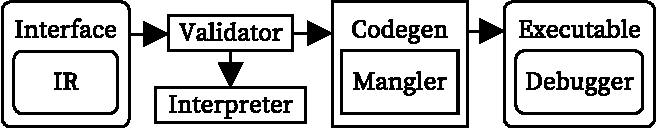
\includegraphics[width=\columnwidth]{overview}

As you can see, the front-end interface contains the Intermediate Representation (IR) and goes through the validator.
From there, depending on the compiler flags, it either goes to the interpreter or the codegen.
In case it goes to the interpreter, the program is directly executed.
In case it goes to the codegen, it is translated to the output language.
To translate all the identifiers, the mangler is needed.
The debugger is optionally embedded in the executable, depending on compiler flags.


\subsection{Output language}
The first research question had the most impact on the project, and was one that was difficult to change later on.

\textit{In what programming language should the code-generator produce its output?}

This may be different than the language the code-generator is written in.
The code-generator is written in F\#, like the rest of the compiler.
The reason we use F\#, rather than Meta-Casanova 2, is because of the debugging capabilities.

\subsubsection{Unmanaged languages}
Since speed was one of the requirements, I first looked at solutions with unmanaged parts.
Unmanaged code is code that is not interpreted by a runtime, but is instead executed directly.
%It is also much less restrictive than the .NET runtime because the .NET bytecode is strongly typed.\cite{ecma335}

The main advantage of unmanaged code is that the fast LLVM code generator can be used.
LLVM is a ``collection of modular and reusable compiler and toolchain technologies.''\cite{llvm}
Specifically, the LLVM optimizer is valuable.
It is used in the Clang, a C/C++ compiler on par with gcc, and with little effort can be use it to optimize our generated code.
This would mean we get all the optimisations of LLVM with relative ease.
It would however mean that we had to implement a garbage collector, as LLVM does not come with one.
 
.NET compatibility is also required, as explained in section \ref{whydotnet}.
There are a few systems that allow for managed and unmanaged code to communicate.
The most viable are P/invoke, C++/CLI interop, and a hosted runtime.

\paragraph{P/invoke}
Platform Invocation Services (P/invoke) allows managed code to call unmanaged functions that are implemented in a DLL.\cite{msdn_pinvoke}

This is the most common form of inter-op, and has great documentation.
However, there are two big disadvantages.

\begin{enumerate}
    \item .NET can only call native functions, not the other way around.
        This means that the bulk of the control flow happens inside .NET, minimizing the fast native code.
    \item Transfering data between .NET and native code has a high performance cost\cite{msdn_interop_performance}, since it has to be serialized.
        This overhead is so large that we expect it to negate any performance benefit from using native code.
\end{enumerate}

Because of this, P/Invoke was not chosen.

\paragraph{C++/CLI interop}
C++ for the Common Language Infrastructure (C++/CLI) is a programming language designed for interoperability with unmanaged code.\cite{msdn_c++cli}

While it seems like it does exactly what we need, it has portability issues.
The only C++/CLI compiler runs on windows and it only compiles for processors with the x86 architecture\cite{mono_c++cli}.
Besides that, non-typesafe operations (the main advantage of C++/CLI) are only allowed on windows.\cite{mono_c++cli}

This means C++/CLI is not cross-platform enough.

\paragraph{Hosted runtime}
It is possible to embed a .NET runtime inside a native program.
This would make it so the control flow takes place inside the native part.

This seems like the best solution out of the native hybrids.
However it still has two drawbacks.
The mono runtime has a different interface than the microsoft .NET api, leading to incompatible programs \cite{mono_embedding}.
The same large serialization overhead as P/Invoke is present\cite{msdn_hosted}.

\paragraph{Unmanaged language conclusion}
None of the inter-op methods offer a satisfactory solution.
They all have downsides that outweigh the benefits.
It was decided to let go of the LLVM code-generation in favor of a more portable and reliable system.

\subsubsection{.NET languages}
Because of the problems with native hybrids, it was decided to choose a .NET language.
Stability is a big advantage because everything happends inside the .NET runtime.
This has a higher chance of working on non-native platforms than the hybrid solutions.

\paragraph{F\#}
F\# is a functional/declarative language in the .Net family\cite[fsharp].
It would be a natural choice, since the compiler is written in it.
However, it is quite slow\cite{fsharp_slow} and resists the imperative style of the generated code.
The programmer has also less control of the program execution, as F\# is a more higher-level language\cite{fsharp}

A version of the code generator was made that used F\#, but it proved too cumbersome since there was no mechanism to simply skip rules if they failed.

% maybe look for Mohammeds compiler written in F#?

\paragraph{C\#}
C\# is an imperative, object-oriented language\cite{csharp}.
It is the most popular .NET language\cite{Meyerovich}, so the compiler gets the most attention by Microsoft.
It is also easy to debug, as it has the most mature debugging tools.

When implementing the code-generator in this style, it was possible to write the code-generator so that the output-code is straight-line code.
This is opposed to F\#, where I had to generate a tree-structure as an output.
This greatly improved debugability and simplicity of implementation.

\paragraph{CIL}
CIL (Common Intermediate Language) is the bytecode that all the languages are compiled to.
Since it is typed, it has the same restrictions as C\#.[source]
As a result, it makes debugging and verification harder, with little to no gain.
It also ommits the optimizations of the C\# compiler, such as dead-code elimination and stuff\cite{csharp_optimizations}.

\paragraph{Managed language conclusion}
The debugability together with a lot of control make C\# the best choice in this case.


\section{The front-end interface}
The front-end interface is the interface between the front-end and the back-end.
It contains all the information the backend needs.
Primarily the lambda and function defenitions, and the data declarations.

\begin{code}
type Interface = {
  datas      : List<Id*Data>
  funcs      : List<Id*List<rule>>
  lambdas    : List<LambdaId*rule>
  main       : rule
  assemblies : List<string> 
  flags      : CompilerFlags
}
\end{code}

The design principles for this interface were simplicity and minimalism.
There should be as few ways as possible to represent the same program.
This makes testing easier and minimizes bugs that appear only in certain representations of the same program.

The reason that datas, funcs and lambdas are defined as a list of key-value pairs instead of as a Map, is that the keys are not guaranteed to be unique.
Since MC allows polymorphic types, one indentifier may be defined multiple times: once for each type.
There is no performance penalty, as no lookups by identifier are performed.

\subsection{Data declarations}
The data declarations are grouped with the identifier of 

\begin{code}
datas : List<Id*Data>
\end{code}

Where \verb|Data| is simply a list of input types and output types.

\begin{code}
type Data = {
  args       : List<Type>
  outputType : Type
}
\end{code}

Where \verb|Type| represents a monomorphic MC type.

%\begin{code}
%type Type 
%  = DotNetType      of TypeId
%  | McType          of TypeId
%  | TypeApplication of Type*List<Type>
%  | Arrow           of Type*Type
%\end{code}

To illustrate, let's define a tuple an a union in MC.

\begin{code}
Data int -> "," -> string -> int * string
Data "fst" -> int    -> int | string
Data "snd" -> string -> int | string
\end{code}

This will appear as the following list in the interface:

\begin{tabular}{lll}
    \textbf{identifier} & \textbf{arguments} & \textbf{type}\\
    \verb:",":   & \verb:int:; \verb:string: & \verb:int * string: \\
    \verb:"fst": & \verb:int:                & \verb:int | string: \\
    \verb:"snd": & \verb:string:             & \verb:int | string: \\
\end{tabular}


\subsection{Rule containers}

Function and lambda definitions, aswell as the main function contain rules.

\begin{code}
  funcs   : List<Id*List<rule>>
  lambdas : List<LambdaId*rule>
  main    : rule
\end{code}

Functions in MC can contain multiple rules that implement them.

The entry-point of the program is defined by a single rule, here called \verb|main|.
It is not a full function since full functions can have multiple rules.
This was done to make the entry-point as simple as possible.

\subsection{Rules}

Rules rules rules.

\begin{code}
type rule = {
  premises    : List<premise*linenr>
  input       : List<local_id>
  output      : local_id
  typemap     : Map<local_id,Type>
  declaration : Position
  definition  : Position
}
\end{code}

At the heart of the rule is the list of premises.
These premises are a simple and orthogonal instructions in SSA form.

--- design of premises here ---

\subsection{Metadata}

All the symbols in the descriptions are provided with monomorphic types by the front-end.
Functions with generic types are made concrete by the front-end.

Rules are represented wi

The AST was developed in co-operation with the front-end developer.

\subsection[Intermediate Representation]{Intermediate\\Representation}\label{ir}
While the intermediate representation (IR) of the functions is part of the interface, it is complex enough to have its own research question.

\textit{What should the intermediate representation of the functions be?}

Each rule contains a list of premises\footnote{see section~\ref{premises}}.
These premises represent the executable code in each rule.

To minimize the number of representations of the same program, all compound premises are split into multiple premises that do only one operation each.
This process is called \textit{normalization}\label{normalization}.

The instruction set exists in two parts: the base instructions and the .NET extentions.

\subsubsection{Base instructions}
The instruction set was designed to minimize the number of representations of the same program.
This happens to coincide with a small orthogonal instruction set.

The instruction set is in \textit{static single assignment} (SSA) form~\cite{leestatic}.
This means the local identifiers are constant and can not be redefined.

Base instructions fall in one of two groups.
The first maps a global identifier to a local identifier.
These are the \textit{Literal} and \textit{Closure} instructions.
The second operates on local identifiers.
The \textit{Conditional}, \textit{Deconstructor}, \textit{Application} and \textit{Call} instructions belong to this group.

\begin{description}
\item[Literal] (\verb|42 -> x|) assigns a string-, boolean-, integer- or floating-point literal to a local identifier.
\item[Conditional] (\verb|x < y|) asserts that a comparison between local identifiers is true.
    The comparisons can be \verb|<|,\verb|<=|,\verb|==|,\verb|>=|,\verb|>| or \verb|!=|.
    If the assertion does not match, the rule does not match and the next rule in the function is attempted.
\item[Deconstructor] (\verb|lst -> x::xs|) disassembles a local identifier constructed by a data declaration.
\item[Closure] (\verb|(+) -> add|) assigns a closure of a global function to a local identifier.
    The closure can hold a function, lambda or data-constructor.
\item[Application] (\verb|add a -> inc|) applies a local identifier to a closure in another local identifier.
\item[Call] (\verb|inc b -> c|) applies a local identifier and calls the closure.
    All closures need to be called eventually to be useful.
    The exception is data-constructors. 
    They do not have to be called as they insert their elements in the datastructure as they are applied.
\end{description}

\subsubsection{.NET extentions}
A separate set of instructions are needed to inter-operate with .NET.
This is because unlike MC, .NET objects are mutable, and the functions can be overloaded on the number and types of arguments.

\begin{tabular}{ll}
    \textbf{instruction} & \textbf{MC example}\\
    call & \begin{lstlisting}
        System.DateTime d m y -> date
    \end{lstlisting}\\
    static call & \begin{lstlisting}
        System.DateTime d m y -> date
    \end{lstlisting}\\
    get & \begin{lstlisting}
        System.DateTime d m y -> date
    \end{lstlisting}\\
    static get & \begin{lstlisting}
        System.DateTime d m y -> date
    \end{lstlisting}\\
    set & \begin{lstlisting}
        System.DateTime d m y -> date
    \end{lstlisting}\\
    static set & \begin{lstlisting}
        System.DateTime d m y -> date
    \end{lstlisting}\\
\end{tabular}

\subsubsection{Evolution}
It was briefly considered to use an existing intermediate representation, like CIL or LLVM-IR.
However, it would mean over 100 instructions and the front-end would do most of the work.
It would also mean the front-end needed its own codegen to generate the CIL instructions.

Call did not used to apply an argument, but it caused inconsistencies in the type-checker.
There would be not difference in the type of the uncalled closure and the called closure, resulting in an extra bit of information being required with the type.
This caused special-cases all over the codebase, so it was decided to make application take an argument, like in lambda-calculus.

Application used to also take the position of the argument that was applied.
This was because the backend did not care in what order the closures were applied.
But since the MC language only allows for in-order closure application, the decision was made to make the position of the argument implicit to limit the program representations.

Comparisons could first only take a boolean local identifier.
It was changed to a predefined set of comparisons because of two reasons.
Firstly, it makes the language-agnostic base instructions depend on .NET Booleans.
Secondly, by restricting the inputs to only a predefined set of comparisons, we restrict the number of representations for the same program.


\subsection{Code generator}
The fourth research question gets at the heart of the back-end.

\textit{How does the intermediate representation map to the output language?}

The codegen is in many ways the heart of the back end, as it is responsible for generating the C\# code.

\subsubsection{Function declarations}
Function

\begin{code}
class #\textit{<function name>}# {
    #\textit{<function arguments>}#
    public #\textit{<return type>}# 
    run(#\textit{<last argument>}#) {
        {
            #\textit{<rule 1 implementation>}#
            return #\textit{<local>}#;
        }
      skip1:
        {
            #\textit{<rule 2 implementation>}#
            return #\textit{<local>}#;
        }
      skip2:
        #\vdots#
        {
            #\textit{<rule n implementation>}#
            return #\textit{<local>}#;
        }
      skip#\textit{n}#:
        throw new #\textit{<exception>}#;
    }
};
\end{code}

\subsubsection{Data declarations}
Data declarations are implemented with inheritance.
The declared type is represented by an empty baseclass and all the constructors inherit from it.

It is easy to see the pattern with an example.

\begin{code}
Data string -> "," -> int -> string * int

Data "Left"  -> string -> string | float
Data "Right" -> float  -> string | float
\end{code}

Transforms into this.

\begin{code}
class _star {};
class _comma { string _arg0; int _arg1;}

class _pipe {};
class _Left :_pipe {string _arg0;};
class _Right:_pipe {float  _arg0;};
\end{code}

\subsubsection{Rules}

Each rule defines its own name for each input argument.
These names do not have to be the same, for example:

\begin{code}
    Func "evenOrOdd" -> int -> string
    
    a%2 = 1
    -----------------
    evenOrOdd a -> "odd!"

    b%2 = 0
    ------------------
    evenOrOdd b -> "even!"
\end{code}

Of course, by the time the code has arived by the codegen, it would already have been normalized.
So the rules actually look more like this:

\begin{code}
    (%) -> _tmp0         #\textit{(closure)}#
    _tmp0 a -> _tmp1     #\textit{(application)}#
    2 -> _tmp2           #\textit{(literal)}#
    _tmp1 _tmp2 -> _tmp3 #\textit{(call)}#
    0 -> _tmp4           #\textit{(literal)}#
    tmp4 = tmp0          #\textit{(conditional)}#
    "even" -> _tmp5      #\textit{(literal)}#
    --------------------
    evenOrOdd a -> _tmp5
\end{code}

\begin{code}
    (%) -> _tmp0         #\textit{(closure)}#
    _tmp0 a -> _tmp1     #\textit{(application)}#
    2 -> _tmp2           #\textit{(literal)}#
    _tmp1 _tmp2 -> _tmp3 #\textit{(call)}#
    1 -> _tmp4           #\textit{(literal)}#
    tmp4 = tmp0          #\textit{(conditional)}#
    "odd" -> _tmp5       #\textit{(literal)}#
    --------------------
    evenOrOdd a -> _tmp5
\end{code}

The first job of the rule is to translate the input arguments to their name and return the output.

\begin{code}
    {
        var a = _arg0; 
        ...
        return _tmp5;
    }
    _skip0:
    {
        var b = _arg0;
        ...
        return _tmp5;
    }
    _skip1:
\end{code}

Then each instruction is generated.

\begin{code}
    {
        var a = _arg0; 
        // closure
        var _tmp0 = new _plus(); 
        // application
        var _tmp1 = add;
        _tmp1._arg0 = a;
        // literal
        var _tmp2 = 2;
        // call
        var _tmp3 = _tmp1.run(_tmp2);
        // literal     
        var _tmp4 = 1;
        // conditional
        if(!(_tmp3=_tmp4)){goto _skip0;}
        // literal
        "odd!" -> _tmp5;
        return _tmp5;
    }
    _skip0:
    {
        var b = _arg0;
        ...
        return _tmp5;
    }
    _skip1:
\end{code}

\end{multicols}
figure 1: \textit{an overview of instruction generation.}\\
\begin{tabular}{lll}
    \hline
    \textbf{instruction} & \textbf{MC} & \textbf{C\#}\\

    \hline
    literal & \begin{lstlisting}
        42 -> x
    \end{lstlisting} & \begin{lstlisting}
        var x = 42;
    \end{lstlisting} \\

    \hline
    conditional & \begin{lstlisting}
        x > 40  
    \end{lstlisting} & \begin{lstlisting}
        if(!(x>40)){goto skip0;}
    \end{lstlisting} \\

    \hline
    destructor & \begin{lstlisting}
        lst -> x::xs 
    \end{lstlisting} & \begin{lstlisting}
        var _tmp0 = lst as _colon_colon;
        if(_tmp0==null){goto _skip0;}
        var x  = _tmp0._arg0;
        var xs = _tmp0._arg1;
    \end{lstlisting} \\

    \hline
    closure & \begin{lstlisting}
        (+) -> add
    \end{lstlisting} & \begin{lstlisting}
        var add = new _plus();
    \end{lstlisting} \\

    \hline
    application & \begin{lstlisting}
        add a -> inc
    \end{lstlisting} & \begin{lstlisting}
        var inc = add;
        inc._arg0 = a;
    \end{lstlisting} \\

    \hline
    call & \begin{lstlisting}
        inc b -> c
    \end{lstlisting} & \begin{lstlisting}
        var c = inc;
        inc._arg1 = b.run();
    \end{lstlisting} \\

    \hline
    .Net constructor & \begin{lstlisting}
        System.DateTime d m y -> date
    \end{lstlisting} & \begin{lstlisting}
        var date = System.DateTime(d,m,y);
    \end{lstlisting} \\

    \hline
    .Net call & \begin{lstlisting}
        date.toString format -> str
    \end{lstlisting} & \begin{lstlisting}
        var str = date.toString(format);
    \end{lstlisting} \\

    \hline
    .Net static call & \begin{lstlisting}
        System.DateTime.parse str -> date
    \end{lstlisting} & \begin{lstlisting}
        var date = System.DateTime.parse(str);
    \end{lstlisting} \\

    \hline
    .Net get & \begin{lstlisting}
        date.DayOfWeek -> day
    \end{lstlisting} & \begin{lstlisting}
        var day = date.DayOfWeek;
    \end{lstlisting} \\

    \hline
    .Net set & \begin{lstlisting}
        hr -> System.DateTime.hour
    \end{lstlisting} & \begin{lstlisting}
        System.DateTime.hour = hr;
    \end{lstlisting} \\

    \hline
\end{tabular}
\pagebreak
\begin{multicols}{2}
 % double width and page-breaking

\subsubsection{Evolution}
C\# unions only work with value-types.


\section{Mangler}
The mangler is responsible for generating a unique C\# identifier for every instance of an MC identifier.
The mangler is designed to be simple, and produce readable output.
Readable output makes it easy to verify both the mangler and the generated code.

There are two kinds of identifier: global identifiers and local identifiers.
Global identifiers have a fully-qualified name with type information, where as local identifiers only have the simple name.

\subsection{C\# identifiers}
Since there are more valid MC identifier names than C\# identifier names, some characters have to be escaped.

Valid C\# identifiers are \verb|[_A-Za-z][_A-Za-z0-9]*| \cite{msdn_identifiers}.
The only valid non-alphanumeric character is an underscore, so that is used to escape with.

The first iteration of the code mangler just replaced all non-numeric characters with an underscore followed with the two-digit hexadecimal number.
This generated correct identifiers but was very unreadable, \verb|>>=| would translate to \verb|_3E_3E_3D|.
To remedy this, every ascii symbol gets a readable label.

\begin{tabular}{ll|ll|ll}
\verb0!0 & \verb0_bang0  & \verb0-0 & \verb0_dash0  & \verb0=0 & \verb0_equal0 \\
\verb0#0 & \verb0_hash0  & \verb0.0 & \verb0_dot0   & \verb0?0 & \verb0_quest0 \\
\verb0$0 & \verb0_cash0  & \verb0/0 & \verb0_slash0 & \verb0@0 & \verb0_at0    \\ %$
\verb0%0 & \verb0_perc0  & \verb0\0 & \verb0_back0  & \verb0^0 & \verb0_caret0 \\
\verb0&0 & \verb0_amp0   & \verb0:0 & \verb0_colon0 & \verb0_0 & \verb0_under0 \\
\verb0'0 & \verb0_prime0 & \verb0;0 & \verb0_semi0  & \verb0`0 & \verb0_tick0  \\
\verb0*0 & \verb0_amp0   & \verb0<0 & \verb0_less0  & \verb0|0 & \verb0_pipe0  \\
\verb0+0 & \verb0_plus0  & \verb0>0 & \verb0_great0 & \verb0~0 & \verb0_tilde0 \\
\verb0,0 & \verb0_comma0 \\
\end{tabular}

\subsection{reserved words}
C\# allows reserved words to be used as valid identifiers if prefixed with an `\verb|@|'\cite{msdn_identifiers}.

\subsection{types}
Global identifiers need type information embedded in the name since the name alone does uniquely identify it (see thingy).
Types can be recursive (see types), so the system for embedding types must be able to represent tree structures.
We use the same syntax as the front-end but with \verb|_S| as seperator, \verb|_L| for the left angle bracket and \verb|_R| for the right angle bracket.

\begin{tabular}{ll}
\textbf{type}          & \textbf{mangled} \\
\verb|array<int,3>|    & \verb|array_Lint_S3_R| \\
\verb|list<list<int>>| & \verb|list_Llist_Lint_R_R| \\
\end{tabular}


\subsection{Interpreter}
The sixth research question lead to the implementation of an interpreter.

\textit{How to validate the code generator?}

The interpreter was built to automatically validate the code generator and later allow constant-folding as a compiler optimization.

The automatic validation would be done by comparing the results of test programs between the interpreter and the compiler.
If they mismatch, there is either a bug in the interpreter or (more likely) a bug in the code generator.

\subsubsection{Evolution}
The first design for an interpreter used the continuation monad.
This is a complex construct that allows for arbitrary control flow.

The idea was that during debugging, you could change the line that was executed.
It turned out that it was more desirable to have the debugger in the code generator instead of the interpreter\footnote{see section \ref{debugger}}, so the primary benefit of the construct was lost.

The next design used explicit recursion to walk the list of instructions.
This was a huge simplification compared to the continuation-monad, but every instruction still had to explicitly recurse over the instruction list.
While all of the recursive calls were tail-calls\cite{tailcalls}, it still meant near-identical code duplication for each instruction.

\subsubsection{Structure}
The final design uses \verb|fold|, a specialization of a catamorphism for lists\cite{catamorphism}.
This eliminated the recursion, making \verb|interpret| a straight-line function that executed a single instruction.
This interpreter was written in under 100 lines\footnote{see \texttt{interpreter.fs}}.

\verb|fold| (or \verb|reduce|) is a standard function in F\# and other functional languages with the following type signature:

\begin{FS}
    fold : (s->a->a) -> s -> [a] -> a
\end{FS}

It applies a function for each element that takes the element and accumulator and produces a new accumulator.
The first argument is that function, the second argument is the starting state and the last is the array.
~\cite{realworldhaskellch4}.

For example: \texttt{fold (+) 0 [1 2 3 4]} evaluates to 10 and \texttt{fold (*) 1 [1 2 3 4]} evaluates to 24.

Using a fold radically simplifies the function, as all the explicit recursion becomes implicit.
The function now only takes the state of the program and an instruction, and produces the new state of the program.

\subsubsection{.NET instructions}
The interpreter has to be able to load .NET libraries on the fly, since the libraries are not known at the time the compiler is compiled.

In the front-end interface, the \verb|assemblies| field contains a list of strings.
These strings are the assembly names the program is linked to.
When a .NET function is called, the interpreter will open the assemblies one by one and search through it for a function that matches the name and signature of the one called.
.NET data structures and fields are handled the same way.


\subsection{Debugger}\label{debugger}
The validation of the codegen lead to another validation-issue.
If a test program is not behaving as expected, is there a bug in the test program or in the compiler?

In other words:

\textit{How to validate the test programs?}

The answer to this is an embedded debugger in the target executable.

\fbox{\includegraphics[width=\columnwidth-7pt]{debugger}}

%The backend can also embed an interactive debugger in the codegen.
The program will then trigger a breakpoint on the first instruction and launch the debugger GUI.
From the GUI, more breakpoints can be set with the check-boxes.
When the user presses `continue' or `abort', the gui will close and appear again on the next breakpoint.

The left pane shows a four level deep tree which sorts the program on file name, function name, rule and line.

The right pane shows a table with the name and value of the local identifiers defined up to the current breakpoint.

\subsubsection{Program changes}
When compiling with the debug flag set, some additions are made to target program.

\paragraph{Local identifier table}
After each instruction that defines named local identifiers, a new instruction is generated.

\begin{code}
    var foo = 42;
    _DBUG_symbol_table["foo"] = foo;
\end{code}

After each assignment to a named local identifier, the named identifier and the value are recorded in a key-value collection. 
This key-value collection will be passed to the debugger when a breakpoint is hit.
A new key-value collection is defined at the start of each rule.

\paragraph{Break points}
When compiling with the debug-flag set, function closures will have a group of boolean arrays.
One array for each rule in the function.

\begin{code}
    class <function name>{
        <arguments>
        static bool[] _DBUG_breakpoints_0;
        static bool[] _DBUG_breakpoints_1;
        <return value> _run(<last argument>){
            <body> 
        }
    }
\end{code}

The breakpoints are generated at each line of sourcecode in the rule.
This is different than breaking at every instruction, as normalization often splits single lines into multiple instructions.

\begin{code}
    ...
    if(_DBUG_Breakpoints_1[6]){
        _DBUG.breakpoint("filename.mc", 12, 
                         _DBUG_symbol_table);
    }
    ...
\end{code}

\subsubsection{Debug class}
The breakpoint function is defined as a public static member of the debug class.

The debugger is defined in a seperate file, \verb|_DBUG.cs|, which is imported by the target executable.
This is done to keep the program-specific code out of \verb|_DBUG.cs|.

\verb|_DBUG.cs| contains the class \verb|_DBUG|.
This class contains only the following public static items.

\begin{enumerate}
    \item the program tree
    \item the breakpoint tree
    \item the breakpoint function
\end{enumerate}

The program builds up the program tree and the breakpoint tree in the main function, before the first user-written line starts.
The trees are both four-levels deep and sorted on filename, function name, rule and linenumber.
The breakpoint function is called when the program hits a break-point.

This was chosen because breakpoint checks happen every few instructions, so they have a huge effect on debug performace.
Straight arrays with booleans are very fast to index since it only costs one bounds-check, one addition and one dereference.

\paragraph{The tree representation} of the program is four levels deep.
The first level represents the file, the second level represents the funcion, the third level represents the rule and the fourth level represents the premise.

\paragraph{The breakpoint table} 
Breakpoints are realised as an array of booleans for each rule in a closure.
The class also contains a \verb|bool[][][][]| 

\paragraph{The breakpoint function}
This class contains a static method \verb|breakpoint| that will pause the execution of the program and present the GUI.
When the user presses `continue' or `abort', the GUI will close and the \verb|breakpoint| method will return control back to the program.

The first two arguments to \verb|_DBUG.breakpoint| are the filename and the linenumber.
This is to uniquely identify the callsite.
The third argument is the symboltable that has been accumulated so far.

\subsubsection{Initialization}
The program tree is a public field of the \verb|_DBUG| class, and is initialized by the main function.

\subsubsection{Evolution}
First own tree impl.
Then 4d node.
Now winform tree nodes.



\section{Results}
The result is a working, reliable, performant back-end, with interpreter, validator and embedded debugger.

To prove it works, three test programs were written.
All are correctly generated, all run in the interpreter, and all can be debugged.

\subsection{Test programs}
Unfortunately, since the front-end was incomplete, it is not possible to compile source files.
It \textit{is} however possible to write the front-end interface by hand.

\subsubsection{Data test}
The first test was developed to test the Data declarations.
It is equivalent to the following mc code.

\begin{MC}
Data int -> "::" -> List -> List
Data "nil" -> List

---------
main -> 0
\end{MC}

\subsubsection{List length test}
The list length program defined a list datastructure and a program to compute its length.
This was used since it uses each basic instruction at least once, as well as matching.
It is equivalent to the following MC code:

\begin{MC}
Data int -> "::" -> List -> List
Data "nil" -> List

Func "length" -> List -> int

---------------
length nil -> 0

lengtht xs -> res
---------------------
length x::xs -> res+1

--------------------------------
main -> length (1::2::3::4::nil)
\end{MC}

Which when executed prints the following on screen.

\begin{lstlisting}
4
\end{lstlisting}

This program can also be debugged with the embedded debugger.

\subsubsection{XNA test}
The second test program was to test the .Net functionality.
It consists of a simple program that modifies XNA datastructures, specifically the \verb|Vector2|.

\begin{MC}
20.0 -> x1
10.0 -> y1
Microsoft.Xna.Framework.Vector2 x1 y1 -> a
20.0 -> x2
10.0 -> y2
Microsoft.Xna.Framework.Vector2 x2 y2 -> b
Microsoft.Xna.Framework.Vector2.+ a b -> c
Microsoft.Xna.Framework.Vector2.Normalize c
y2 -> v.x 
v.x -> ret
-------------------------------------------
run -> ret
\end{MC}

Which returns \verb|20|.
This is especially intresting to debug, because we can see the values change.

\fbox{\includegraphics[width=\columnwidth-7pt]{debugger}}


\section{Recommendations}

\section{Conclusion}

\subsection{Results}

\section{Reflection}

\section{Further work}\label{recommendations}
The back-end is in a functional state, but it could use more features.
Most of the features are optimizations.
Because the performance requirement was already met, the implementation of these optimizations was not necessary.

\subsubsection{Inlining}
The most important optimization is inlining~\cite{inlining}.
Inlining is the process of replacing a function call with the function body.
While this saves a function call, the greatest benefit is that it enables other optimizations.

When the function body is copied in the larger context of the callsite, some input values may be identified as compile-time constants, enabeling a whole array of optimizations. 

Inlining is not always desireable.
If a large function is called from many different places, the size of the program increases, increasing the cache-misses on the instruction cache, reducing performance.

The choice for inlining a call should consider:
\begin{enumerate}
    \item If the function recurses in any way, even indirect recursion.
        This makes inlining impossible.
    \item The size of the function.
        The smaller the function, the greater the inlining benefit.
    \item The ammount of times the function is called.
        If the function is only called once, inlining has no disadvantages.
        For each additional time, the size of the program increases.
\end{enumerate}

\subsubsection{Tail call optimization}
Some recursive functions can be transformed into loops.
This has the advantage that no new stackframes will be allocated, preventing stack-overflows and increasing performance.

If the function returns right after the recursive call, there is no need to save the state of the function, since it will be thrown away right after the call returns.
In these cases, it is safe to replace the recursion with a modification of the input arguments and a jump to the top of the function.

These constructs can be implemented in C# using \verb|goto|.
Alternatively, the \verb|tail call| CIL instruction can be generated.

\subsubsection{Constant folding}
Constant folding is done when the an expression involving constants can be computed to another constant.
For example the expression \verb|3+5| has only constants in it and can on compile-time be substituted with \verb|8|. 

C\# does constant folding in very limited conditions.
The C\# language specification\footnote{second bullet point of section 11.1.4, page 110 of~\cite{csharp_spec}} states that this is only done on \textit{simple type constants}.
Simple types are types like \verb|int|, \verb|float|, \verb|bool|, \verb|byte| and the like.
Simple types do not include any compound types like structs or classes.
The constant expression can also only be with operators defined by the simple types.
No user-defined function can therefore be constant folded.

The MC compiler could constant fold a lot more.
Everything in a rule that is not related to its inputs can be constant folded.


\section{Evaluation}\label{evaluation}
In this section I will show that I have the competentions associated with computer science according to Rotterdam University of applied sciences.

\subsubsection{Analyzing}


\subsubsection{Designing}
The parts of the back end are modular and communicate with eachother through well-defined interfaces.

\subsubsection{Administering}

\subsubsection{Advizing}

\subsubsection{Realizing}
I managed to to realize a working compiler within the allocated time.



\printbibliography
\end{multicols}
\newpage

% appendix
\setcounter{section}{0}
\renewcommand\thesection{\Alph{section}}

%\section{Stakeholders}
\begin{tabular} { l l }
    \textbf{Student} & \\
    Name & Douwe van Gijn \\
    Student number & 0864504 \\
    E-mail address & 0864504@hr.nl \\
    Telephone number & +31 6 46 909 730 \\
    & \\
    \textbf{Client} & \\
    Name company & Kennis Centrum Creating 010 \\
    Name company supervisor & Sunil Choenni \\
    E-mail address & h.choenni@hr.nl \\
    Telephone number & +31 6 48 10 03 01  \\
    Function & Lector \\
    Visitors address & Wijnhaven 103 floor 6 \\
    Website company & www.creating010.com \\
    & \\
    \textbf{Company supervisor} & \\
    Name company & Kennis Centrum Creating 010 \\
    Name company supervisor & Sunil Choenni \\
    E-mail address & h.choenni@hr.nl \\
    Telephone number & +31 6 48 10 03 01  \\
    Function & Lector \\
    Visitors address & Wijnhaven 103 floor 6 \\
    Website company & www.creating010.com \\
    & \\
    \textbf{School supervisors} & \\
    Name examinator (first teacher) & Giuseppe Maggiore \\
    E-mail address & +31 6 41 78 12 23 \\
    Telephone number & g.maggiore@hr.nl \\
    & \\
    Name assessor (second teacher) & Hans Manni \\
    E-mail address & j.p.manni@hr.nl \\
    Telephone number & \\
    & \\
    \textbf{School coördinator} & \\
    Name graduate coördinator INF/TI & Aad van Raamt \\
    Telephone number & 010 7944993 \\
    E-mail address & A.van.Raamt@HRO.NL \\
\end{tabular}
\newpage


%\begin{multicols*}{2}
%\section{Glossary}
%\begin{description}
%    \item[boilerplate code] expl
%    \item[polymorphic] can have multiple types
%\end{description}
%\end{multicols*}
%\newpage

\section{Benchmarks}
\subsection{list.cs}
\lstinputlisting[numbers=left,language=CSharp]{sourcefiles/list.cs}
\subsection{list.py}
\lstinputlisting[numbers=left,language=Python]{sourcefiles/list.py}
\subsection{native.py}
\lstinputlisting[numbers=left,language=Python]{sourcefiles/native.py}

%\section{Source code}
%\subsection{Common.fs} 
%\lstinputlisting[numbers=left,language=FSharp]{sourcefiles/Common.fs}
%\subsection{CodegenInterface.fs} 
%\lstinputlisting[numbers=left,language=FSharp]{sourcefiles/CodegenInterface.fs}
%\subsection{Interpreter.fs} 
%\lstinputlisting[numbers=left,language=FSharp]{sourcefiles/Interpreter.fs}
%\subsection{Codegen.fs} 
%\lstinputlisting[numbers=left,language=FSharp]{sourcefiles/Codegen.fs}
%\subsection{Mangle.fs} 
%\lstinputlisting[numbers=left,language=FSharp]{sourcefiles/Mangle.fs}
%\subsection{\_dbug.cs}
%\lstinputlisting[numbers=left,language=CSharp]{sourcefiles/_dbug.cs}
%\subsection{Listtest.fs} 
%\lstinputlisting[numbers=left,language=FSharp]{sourcefiles/listtest.fs}
%\subsection{Balltest.fs} 
%\lstinputlisting[numbers=left,language=FSharp]{sourcefiles/balltest.fs}

\end{document}
